\subsection{Debugger}\label{debugger}
The validation of the codegen lead to another validation-issue.
If a test program is not behaving as expected, is there a bug in the test program or in the compiler?

In other words:

\textit{How to validate the test programs?}

The answer to this is an embedded debugger in the target executable.

\fbox{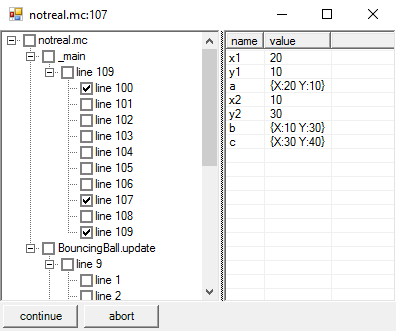
\includegraphics[width=\columnwidth-7pt]{debugger}}

The backend can also embed an interactive debugger in the codegen.
The program will then trigger a breakpoint on the first instruction and launch the debugger GUI.
From the GUI, more breakpoints can be set with the check-boxes.
When the user presses `continue' or `abort', the gui will close and appear again on the next breakpoint.

On the left pane is a 4-level deep tree which sorts the program on file name, function name, rule and line.

On the right pane shows a table with the name and value of the local identifiers defined up to the current breakpoint.

\subsubsection{Debug class}

A seperate file, \verb|_DBUG.cs| contains the class \verb|_DBUG|.
This class contains only the following public static items.

\begin{enumerate}
    \item the tree representation of the program
    \item a breakpoint table
    \item a breakpoint function
\end{enumerate}

\subsubsection{Usage}

--- IM NOT SURE HOW TO STRUCTURE THE REST OF~\ref{debugger} ---

%This class contains a static method \verb|breakpoint| that will pause the execution of the program and present the GUI.
%When the user presses `continue' or `abort', the GUI will close and the \verb|breakpoint| method will return control back to the program.

The class also contains a \verb|bool[][][][]| 

The breakpoints are generated at each line of sourcecode in the rule.
This is different than breaking at every instruction, as normalisation often splits single lines into multiple instructions.

Breakpoints are realised as an array of booleans for each rule in a closure.

\begin{code}
    class <function name>{
        <arguments>
        static bool[] _DBUG_breakpoints_0;
        static bool[] _DBUG_breakpoints_1;
        <return value> _run(<last argument>){
            <body> 
        }
    }
\end{code}

This was chosen because breakpoint checks happen every few instructions, so it has a big performance impact.
Straight arrays with booleans are very fast to index since it only costs one addition and one dereference.

\begin{code}
    ...
    if(_DBUG_Breakpoints_1[6]){
        _DBUG.breakpoint("filename.mc", 12, 
                         _DBUG_symbol_table);
    }
    ...
\end{code}

The first two arguments to \verb|_DBUG.breakpoint| are the filename and the linenumber.
This is to uniquely identify the callsite.
The third argument is the symboltable that has been accumulated so far.

After each assignment to a named local identifier, the named identifier and the value are recorded in a key-value collection. 
This key-value collection will be passed to the debugger when a breakpoint is hit.

\subsubsection{Initialization}
The \verb|_DBUG| class is initialized in the main function.
This is done to keep the program-specific code out of \verb|_DBUG.cs|.
The program tree is a public field of the \verb|_DBUG| class, and is initialized by the main function.

